	\begin{apendicesenv}
	
	% Imprime uma página indicando o início dos apêndices
	\partapendices
	\chapter{Mais detalhes sobre os experimentos}
			\begin{center}
	\newcommand{\mc}[3]{\multicolumn{#1}{#2}{#3}}
	\definecolor{tcB}{rgb}{0.447059,0.74902,0.266667}
	\definecolor{tcA}{rgb}{0.65098,0.65098,0.65098}
	\definecolor{tcC}{rgb}{0,0.8,1}
	
	\begin{longtable}[h]{|c|c|c|c|c|}
		
		% Columns headers
		\hline
		\mc{1}{|>{\columncolor{tcA}}c|}{Mel/Bark}&\mc{1}{|>{\columncolor{tcA}}c|}{Wavelet}&\mc{1}{|>{\columncolor{tcA}}c|}{G1}&\mc{1}{|>{\columncolor{tcA}}c|}{G2}&\mc{1}{|>{\columncolor{tcA}}c|}{Distância de (1,0)}\\\hline
		\endfirsthead
		
		\mc{3}{c}{{\tablename\ \thetable : Continuação da página anterior}} \\\hline
		% Columns headers
		\mc{1}{|>{\columncolor{tcA}}c|}{Mel/Bark}&\mc{1}{|>{\columncolor{tcA}}c|}{Wavelet}&\mc{1}{|>{\columncolor{tcA}}c|}{G1}&\mc{1}{|>{\columncolor{tcA}}c|}{G2}&\mc{1}{|>{\columncolor{tcA}}c|}{Distance to (1,0)}\\\hline
		\endhead
		
		\hline \mc{2}{c}{{Continua na próxima página}} \\
		\endfoot
		\endlastfoot
		
		% Color of the first line
		\rowcolor{tcB}
		
		% Loads data from tables/results/paraconsistentPlane/distParacomFrom10.csv
		\csvreader[
		no head,
		late after line=\\\hline\rowcolor{tcC},%
		separator=comma,
		filter={\value{csvrow}<4},
		]{../monography/tables/results/paraconsistentPlane/distParacomFrom10.csv}{
			1=\melBark,
			2=\wavelet,
			3=\gOne,
			4=\gTwo,
			5=\distance
		}{
			\melBark&
			\wavelet&
			\StrSubstitute[0]{\gOne}{.}{,}&
			\StrSubstitute[0]{\gTwo}{.}{,}&
			\StrSubstitute[0]{\distance}{.}{,}
		}
		
		\rowcolor{white}
		\caption{As 5 primeiras combinações Wavelet \textit{x} Mel/Bark ordenadas pela distância do vértice (1,0) no plano paraconsistente.}
		\label{tab:distParacomFrom10BarkAndMel}
	\end{longtable}
\end{center}
			\begin{landscape}
					\begin{figure}[h]
						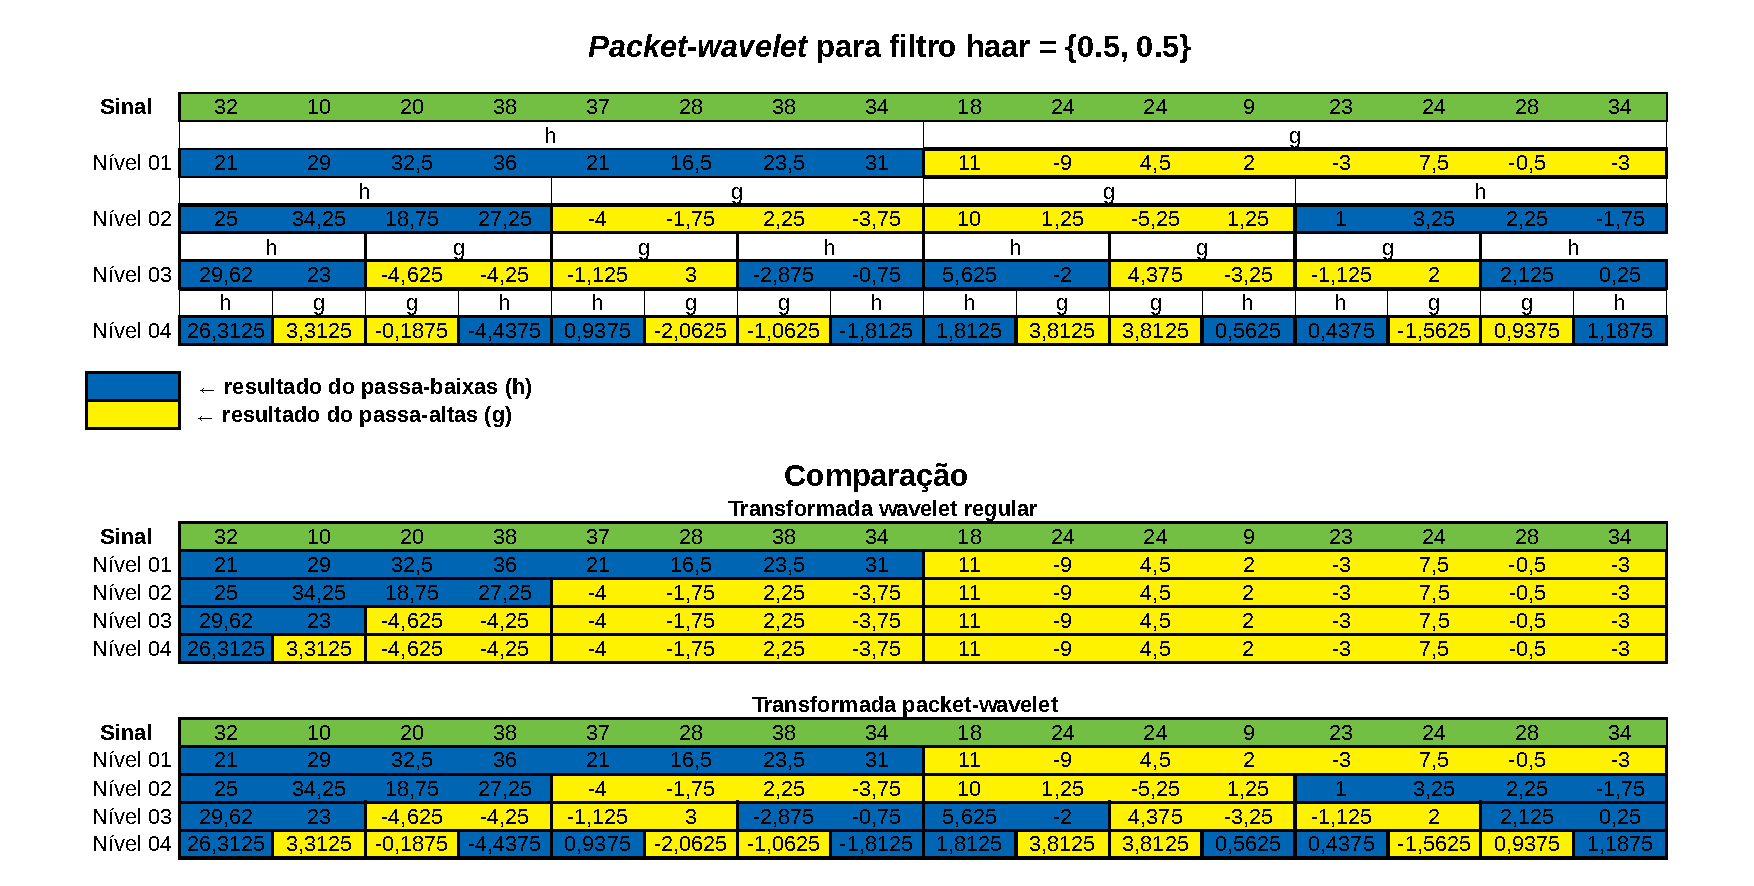
\includegraphics[width=1\linewidth]{images/haarWaveletExamples.pdf}
						\caption{Demostração numérica das transformadas Wavelet e Wavelet packet}
						\label{fig:haarWaveletExamples}
					\end{figure}
			\end{landscape}
			\begin{figure}[h]
				\centering
				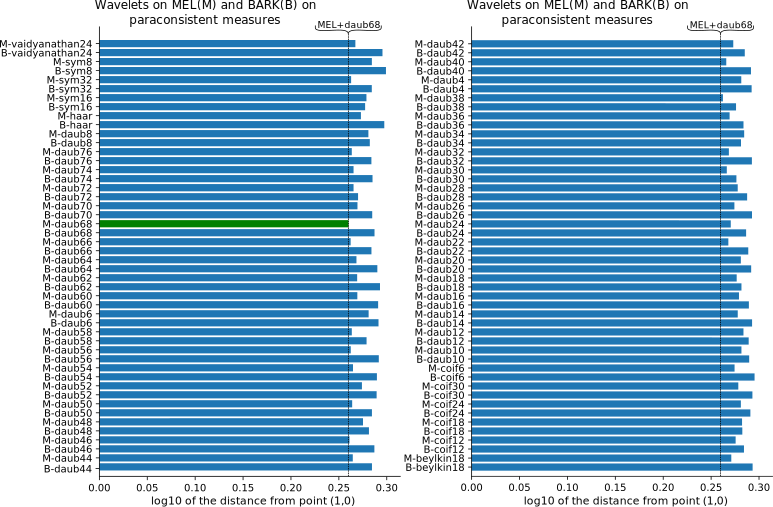
\includegraphics[width=0.99\linewidth]{images/results/paraconsistentPlane/ParaconsistentFull}
				\caption{Gráfico completo da distância ao ponto (1,0) no plano paraconsistente.}
				\label{fig:paraconsistentfull}
			\end{figure}
	\chapter{Recursos na web}
		\par Para realização deste trabalho foram produzidos variados textos (este incluso) e códigos. 
		\par Todos os materiais estão disponíveis em:  \href{https://github.com/ensismoebius/mestrado}{https://github.com/ensismoebius/mestrado}.
\end{apendicesenv}